{\chapter{Evaluation Environment}
\label{chap:Eval_4}

In (\ref{chap:PhysicalDesign}), we have introduced the physical design of a set of graph data structures. We have complemented the implementation of the graph data structures with other components in order to set up a complete environment for evaluating the behaviour of the graph data structures in different scenarios. 

In this chapter, we introduce the details of every component in the evaluation environment which we will use to evaluate our implemented graph data structures. This chapter is consisted of the following sections:

\begin{itemize}  

\item \textbf{Technical Environment:}\\
In \ref{sec:techEnv}, we detail the specifications of the technical environment that we use to test the performance of loading and querying the graph data structures. 

\item \textbf{Evaluation Dataset:}\\
In this section, we present the dataset we used to evaluate the performance of the graph data structures. (\ref{sec:dataset})

\item \textbf{Data Loader:}\\
Next, we present the data loader component that we utilize for loading the data into the graph data structures. (\ref{sec:dataLoader})

\item \textbf{Queries:}\\
In (\ref{sec:qryDef}), we define a set of queries that we perform against the data which we loaded into the graph data structures.

\item \textbf{Summary:}\\
Lastly, we provide a summary for what we discussed in the chapter. (\ref{sec:Eval4-summary})

\end{itemize}


\section{Technical Environment}
\label{sec:techEnv}

In this section, we list the specifications of the technical hardware and software we used to implement, test and evaluate the graph data structures.

Following are the details of the programming language we have used in implementation:

\begin{itemize}
\item Programming language: \texttt{C++}
\item Compiler: \texttt{g++}
\item Compiler version: \texttt{5.5.0}
\end{itemize}

The specifications of the operating system for the test and evaluation machine are below:

\begin{itemize}
\item Operating System: \texttt{Linux}
\item Distribution: \texttt{Ubuntu}
\item Version: \texttt{18.04 LTS}
\item Code Name: \texttt{Bionic Beaver}
\end{itemize}

Lastly, we list the hardware specifications of the test and evaluation machine below:

\begin{itemize}
\item Hardware Provider: \texttt{Microsoft Azure Cloud}
\item Machine Code: \texttt{E16S\_V3}
\item Processor: \texttt{Intel(R) Xeon(R) CPU E5-2673 v4}
\item Processor Speed: \texttt{2.30GHz}
\item Number of Cores: \texttt{16}
\item Main Memory: \texttt{128 GiB}
\end{itemize}

\section{Evaluation Dataset}
\label{sec:dataset}

For evaluating the implemented graph data structures, we have used a dataset that we have generated using the \textit{Linked Data Benchmark Council} (LDBC) - \textit{Social Network Benchmark} (SNB) framework \cite{boncz2013ldbc, prat2017ldbc}.

\begin{figure}[hbtp]
\centering
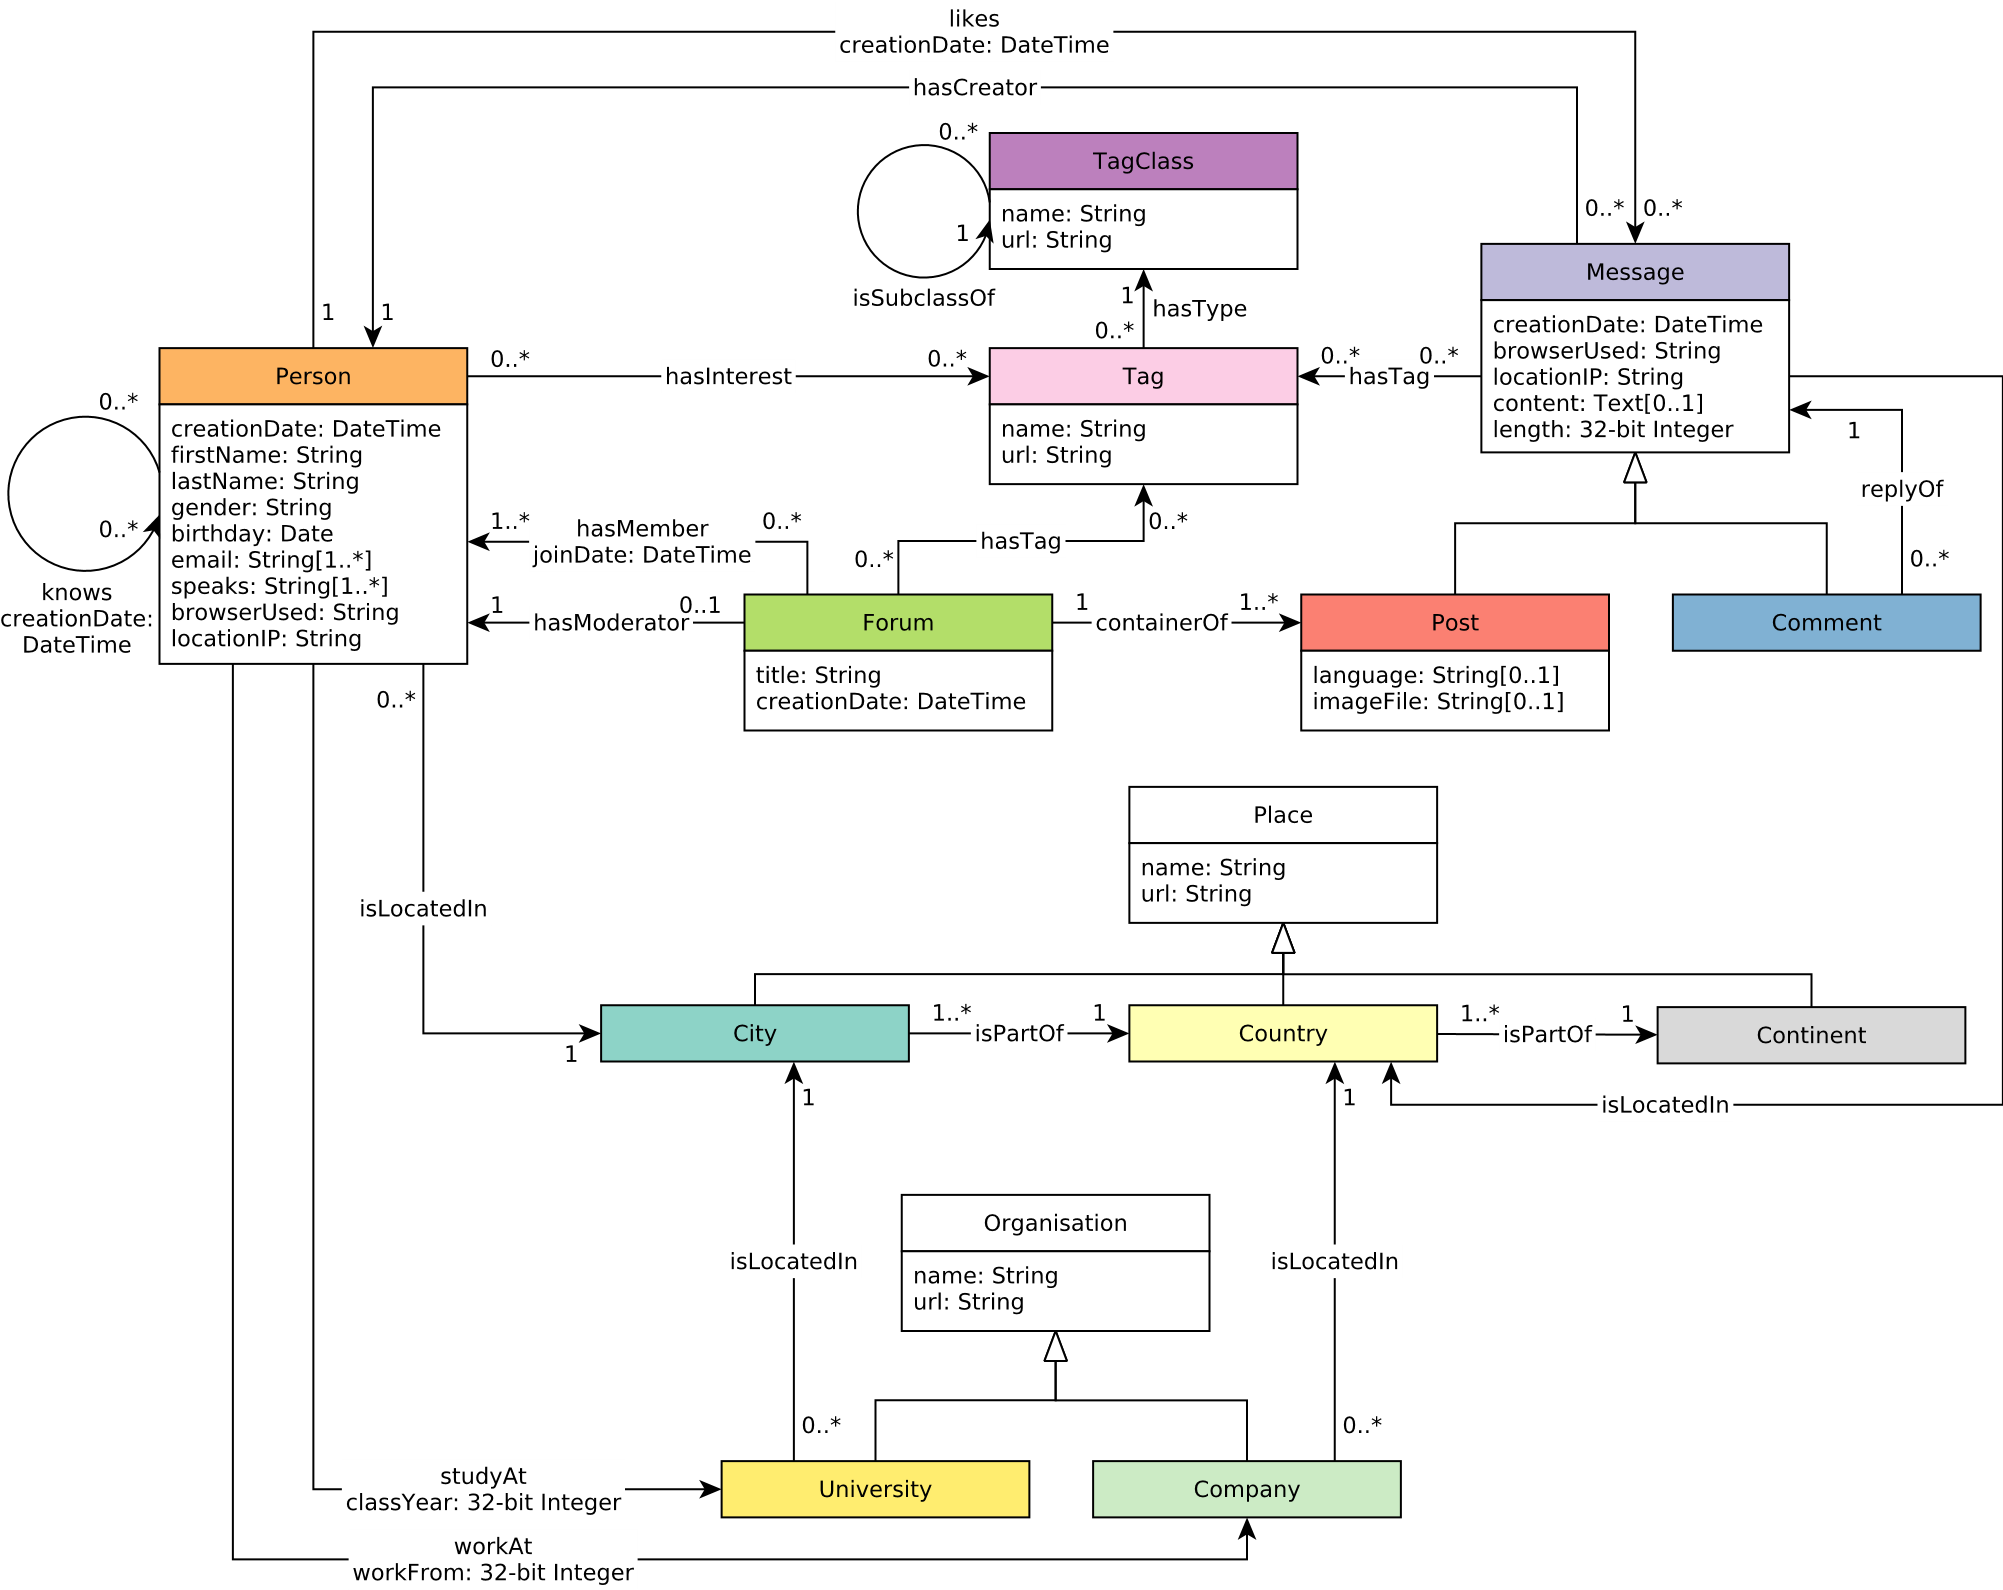
\includegraphics[width=1\textwidth]{pics/LDBC.png}
\caption{LDBC - SNB data model \cite{prat2017ldbc}.}
\label{fig:LDBC-DataModel}
\end{figure} 

The Linked Data Benchmark Council (LDBC) is an independent non-profit company which focuses on developing of new benchmarks for large-scale graph and RDF data management, establishing an industry-neutral entity for developing graph and RDF benchmarks, auditing benchmark results, and publishing audited results \footnote{For more information on the Linked Data Benchmark Council - Social Network Benchmark framework see:  http://ldbc.github.io/ldbc\_snb\_docs/ldbc-snb-specification.pdf}.

The LDBC - Social Network Benchmark (SNB) framework is providing a data generator that generates a synthetic
social network data. The data generator produces networks with described schema with distributions and correlations similar to those expected in a real social network. The schema represents a realistic social network, including people and their activities in the social network during a period of time. In (\ref{fig:LDBC-DataModel}), we show a UML diagram for the data model of the LDBC - SNB generated data \cite{prat2017ldbc}.

We have used the LDBC - SNB data generator to generate datasets with different sizes. All the generated datasets are of the same schema shown in (\ref{fig:LDBC-DataModel}). The size of the dataset generated is depending on two parameters provided to the data generator: the number of persons and the number of years. We have generated datasets of different sizes by changing the parameter value of the number of persons while fixing the number of years parameter value. The generated datasets size and parameters are shown in (\ref{tbl:LDBC-DatsetsScales}). We have assigned each generated dataset a scale factor. A scale factor is an indicator of the value of the "\textit{number of persons}" parameter we have used to generate the dataset. For example, a dataset with scale factor 0.25 was generated with a "\textit{number of persons}" parameter of 2500 and a dataset with scale factor 0.5 was generated with a "\textit{number of persons}" parameter of 5000. Similarly, we have assigned scale factors to the other generated datasets \cite{prat2017ldbc}.

% Please add the following required packages to your document preamble:
% \usepackage{booktabs}
% \usepackage{multirow}
% \usepackage{graphicx}
% \usepackage[table,xcdraw]{xcolor}
% If you use beamer only pass "xcolor=table" option, i.e. \documentclass[xcolor=table]{beamer}
\begin{table}[h]
\centering
\resizebox{\textwidth}{!}{%
\begin{tabular}{@{}|l||l|l||l|l|l|@{}}
\toprule
\multicolumn{1}{|c||}{{\color[HTML]{000000} }} & \multicolumn{2}{c||}{{\color[HTML]{000000} Size}} & \multicolumn{3}{c|}{{\color[HTML]{000000} Parameters}} \\ \cmidrule(l){2-6} 
\multicolumn{1}{|c||}{\multirow{-2}{*}{{\color[HTML]{000000} Scale Factor}}} & {\color[HTML]{000000} \# of Vertices} & {\color[HTML]{000000} \# of Edges} & {\color[HTML]{000000} \# of persons} & {\color[HTML]{000000} \# of Years} & {\color[HTML]{000000} Start Year} \\ \midrule
0.25 & 542,040 & 2,634,240 & 2,500 & 3 & 2010 \\ \midrule
0.5 & 1,244,969 & 6,393,902 & 5,000 & 3 & 2010 \\ \midrule
1 & 2,856,994 & 15,530,170 & 10,000 & 3 & 2010 \\ \midrule
2 & 6,509,804 & 36,771,980 & 20,000 & 3 & 2010 \\ \midrule
4 & 14,737,719 & 84,895,633 & 40,000 & 3 & 2010 \\ \bottomrule
\end{tabular}%
}
\caption{The generated datasets size and parameters}
\label{tbl:LDBC-DatsetsScales}
\end{table}

The evaluation dataset is consisted of vertex files and edge files. A vertex file contains data for all the vertices labeled with the same vertex-label. Each line in a vertex file is consisted of a comma-separated list of all the properties describing one vertex. Similarly, an edge file contains data for all the edges labeled with the same edge-label. Each line in an edge file is consisted of all properties describing one edge.

\section{Data Loader}
\label{sec:dataLoader}

In (\ref{sec:dataset}), we presented the dataset we are using to evaluate the performance of the different graph data structures. In this section, we present the data loader component that we used to load the evaluation dataset into the graph data structures.

In (\ref{subsec:batchLoading}), we introduce the data loader that we developed and used to load the evaluation dataset in batches. In (\ref{subsec:parallellLoading}), we introduce the parallel loader that we developed and utilized to load the evaluation dataset in parallel.


\subsection{Batch Loading}
\label{subsec:batchLoading}

We developed the batch data loader in order to pre-process the evaluation dataset, divide the dataset into batches, and load the batches into the graph data structures. Since the vertices files are containing no information regarding the relationships between the vertices, we load the vertices files contents only into the graph properties structures. Meanwhile, we load the edges files into both: the graph topology structures and the graph properties structures.\newline


\definecolor{codeblack}{rgb}{0,0,0}
\definecolor{backcolour}{rgb}{0.95,0.95,0.95}
\definecolor{codegray}{rgb}{0.5,0.5,0.5}

\lstdefinestyle{mystyle}{
    backgroundcolor=\color{backcolour}, 
    keywordstyle=\bold,
    numberstyle=\color{codegray},
    basicstyle=\footnotesize,
    breakatwhitespace=false,         
    breaklines=true,                 
    captionpos=b,                    
    keepspaces=true,                 
    numbers=left,                    
    numbersep=5pt,                  
    showspaces=false,                
    showstringspaces=false,
    showtabs=false,                  
    tabsize=2
}
 
\lstset{style=mystyle}


\begin{lstlisting}[language=C++, caption=Function used for batch loading of data files., label=BatchDataLoader]
void batchLoad(list dataFiles, int batchSize, 
     GraphStruct graphStructure) 
{
       
    Buffer buffer(batchsize);

    for (auto file : dataFiles) 
    {
        for (auto dataLine : file) 
        {

            GraphElement x = parse(dataLine);
            x.setLabel(file.name);
            buffer.insert(x);

            if (buffer.isFull()) 
            {
                graphStructure.consume(buffer);
                buffer.clear();
            }
        }
    }
}

\end{lstlisting}

In (\ref{BatchDataLoader}), we show a simplified version of the function that we developed to batch load the data files into the graph data structures. First, the function is creating a buffer structure with a size equal to the batch size. Next, the batch loader function is iterating over all the files. In (Line 12), the (\texttt{parse}) function  is used to parse each of the data lines in each and every file. The (\texttt{parse}) function is converting a data line into a (\texttt{GraphElement}) object that contains the list of values in the data line. A (\texttt{GraphElement}) object can be casted into a vertex or an edge object depending on the file being loaded if it is a vertices file or an edges file. The name of the file is used as the label of the (\texttt{GraphElement}) object. Next, the (\texttt{GraphElement}) object is inserted into the buffer. The function is checking the buffer to see if it has reached its full capacity. If the buffer is full, the contents of the buffer is consumed by the graph structure and the buffer is cleared.

\subsection{Parallel Loading}
\label{subsec:parallellLoading}

We developed a parallel data loader in order to load the evaluation dataset in parallel. The parallel data loader is creating multiple threads that loads a data file in parallel, therefore the parallel data loader is only valid for use along with the parallel versions of the graph data structures presented in (\ref{sec:PhyDesign-ParallelGraphStructs}). 

A data file is divided into a number of partitions equal to the number of threads. Each thread loads one partition of a data file in parallel with other threads. Each thread is loading its part of the file in the same way the batch data loader is loading the data into the graph data structures. 

Each thread uses a buffer for temporary storage of data. The buffer size is the same across all the threads. Each thread iterates over the data lines located in its assigned partition of the file. The thread parses the data line to construct a vertex or an edge object depending on the file being loaded if it is a vertices file or an edges file. The name of the file is used as the label of the object. Next, the object is inserted into the buffer. The thread is checking the buffer to see if it has reached its full capacity. If the buffer is full, the contents of the buffer is consumed by the graph structure and the buffer is cleared.

\section{Queries}
\label{sec:qryDef}

In (\ref{sec:dataLoader}, we have presented the data loader component which we utilized in order to load the evaluation dataset into the graph data structures. In this section, we present the definition of a set of queries as another component of the evaluation environment. We will use the set of queries presented in this section to evaluate the graph data structures performance in executing each query. 

We present the definition of three different in (\ref{subsec:qry1}, \ref{subsec:qry2}, and \ref{subsec:qry3}). We will define each of the steps required to execute each query and the format of the output that we expect to receive.

The two queries presented in (\ref{subsec:qry1} and \ref{subsec:qry2}) are pattern-matching queries. A pattern matching query is defined as a set of patterns that needs to be matched against the graph elements (vertices and edges) in order to retrieve all elements that match the given pattern.

The query presented in (\ref{subsec:qry3}) is a degree centrality query. In this query we are not matching the graph elements against given patterns, but we are computing the a degree centrality of each vertex in a graph. The degree centrality of a vertex is computing how many edges (incoming and outgoing) the vertex has. The output of the query is a summary report of the degree centrality of all the vertices in the given graph.

\subsection{Query \#1}
\label{subsec:qry1}

The query we present in this section (Query \#1) was introduced as part of the business intelligence workload in the LDBC - Social Network Benchmark (SNB) specification. The query is given the code (\textit{BI 1}) in the specification \cite{prat2017ldbc}. 

Query \#1 is an example of a simple pattern-matching query that requires no traversals between the graph elements. We present in (\ref{fig:Query1}), the pattern which the query matches against all graph elements loaded from the evaluation dataset in (\ref{sec:dataset}). The query is taking one parameter "\textit{\$date}" which is a date parameter. The query checks all the vertices in the graph that have a vertex-label "\textit{Message}" and selects only those having the value of their "\textit{creationDate}" property less than the given date "\textit{\$date}" \cite{prat2017ldbc}.

The set of messages found are then grouped by three levels of grouping \cite{prat2017ldbc}:

\begin{enumerate}

\item By the year part of the "\textit{creationDate}" property.
\item Per each year, group by the message type "\textit{isComment}". The "\textit{isComment}" property computed for each message is set to "\textit{true}" if the message is a comment, "\textit{false}" otherwise.
\item Per each year-message type group, group by the "\textit{lengthCategory}" of each a message. The "\textit{lengthCategory}" of a message is computed based on the "\textit{length}" of each message as following:
\begin{itemize}
    \item "\textit{0}": 0 <= "\textit{length}" < 40 
    \item "\textit{1}": 40 <= "\textit{length}" < 80 (one liner)
    \item "\textit{2}": 80 <= "\textit{length}" < 160 (tweet)
    \item "\textit{3}": 160 <= "\textit{length}" (long)\\
\end{itemize}

\end{enumerate}

\begin{figure}[H]
\centering

\includegraphics[width=1\textwidth]{pics/Query1.png}
\caption{Query \#1 pattern \cite{prat2017ldbc}.}
\label{fig:Query1}
\end{figure} 


The result of the query after grouping will be consisted of the following attributes \cite{prat2017ldbc}:

\begin{enumerate}
\item "\textit{year}": Year part of the "\textit{creationDate}" of a message.
\item "\textit{isComment}": "\textit{true}" if the message is a comment, "\textit{false}" if a post.
\item "\textit{lengthCategory}": "\textit{0}" for short, "\textit{1}" for one-liner, "\textit{2}" for tweet, "\textit{3}" for long.
\item "\textit{messageCount}": Total number of messages in a group.
\item "\textit{averageMessageLength}": Average "\textit{length}" of messages in a group.
\item "\textit{sumMessageLength}": Sum of "\textit{length}" of all messages in a group.
\item "\textit{percentageOfMessages}": "\textit{messageCount}" of a group as a percentage of all messages created before the given date "\textit{\$date}".

\end{enumerate}

Lastly the result set is sorted in the following order \cite{prat2017ldbc}:

\begin{enumerate}

\item \textit{year}: Descending.
\item \textit{isComment}: Ascending.
\item \textit{lengthCategory}: Ascending.

\end{enumerate}


\subsection{Query \#2}
\label{subsec:qry2}

The query presented in this section (Query \#2) was introduced as part of the business intelligence workload in the LDBC - Social Network Benchmark (SNB) specification. The query is given the code (\textit{BI 18}) in the specification \cite{prat2017ldbc}. 

In contrast to Query \#1 which we presented in (\ref{subsec:qry1}), Query \#2  is an example of a more complex pattern-matching query that requires traversals between the graph elements in order to fulfill the query requirements. We present in (\ref{fig:Query2}), the pattern which the query (Query \#2) matches against all graph elements loaded from the evaluation dataset in (\ref{sec:dataset}). The query is taking three parameters as part of the input. The "\textit{\$date}" parameter which is a date, the "\textit{\$lengthThreshold}" parameter which is a number, and the "\textit{\$languages}" parameter which is a list of language-codes. The query checks all the vertices in the graph that have a vertex-label "\textit{Person}" and computes how many messages they made "\textit{messageCount}". The "\textit{Person}" created a "\textit{Message}" is identified as the target vertex of the edge with a label "\textit{hasCreator}" of each "\textit{Message}" \cite{prat2017ldbc}.

\begin{figure}[ht]
\centering
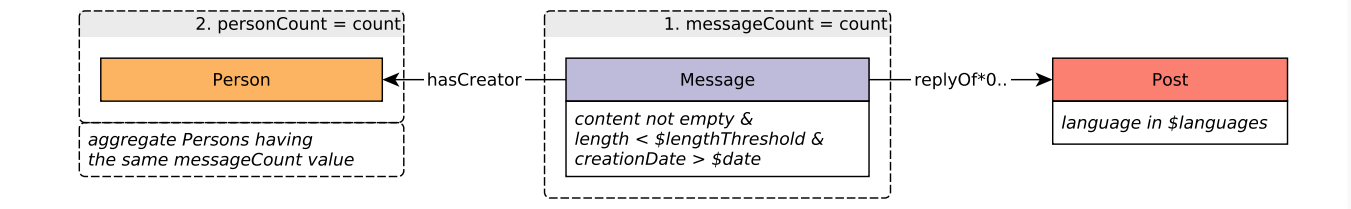
\includegraphics[width=1\textwidth]{pics/Query2.png}
\caption{Query \#2 pattern \cite{prat2017ldbc}.}
\label{fig:Query2}
\end{figure} 

The query counts a "\textit{Message}" only if the message's properties match the following conditions \cite{prat2017ldbc}:

\begin{itemize}

    \item The value of the message's "\textit{content}" property is not empty.
    \item The value of the message's "\textit{length}" property is less than the value of the "\textit{\$lengthThreshold}" parameter.
    \item The value of the message's "\textit{creationDate}" property is less than the value of the "\textit{\$date}" parameter.
    \item The message's language-code is one of the language-codes provided in the "\textit{\$languages}" parameter.
    
    \begin{itemize}
    
    \item The "\textit{language}" property of a "\textit{Post}" identifies its language-code. 
    \item The language-code of a "\textit{Comment}" is defined in \cite{prat2017ldbc} as "that of the "\textit{Post}" that initiates the thread where the "\textit{Comment}" replies to". The Post and Comments in between the "\textit{Comment}" and the root "\textit{Post}" of the thread do not have to meet any condition except for their "\textit{language}".
    
    \end{itemize}
    
\end{itemize}

Next, we group the result set by the "\textit{messageCount}" computed attribute, so that for each unique "\textit{messageCount}", the number of persons who have created the same "\textit{messageCount}" of messages are counted \cite{prat2017ldbc}.

The final result set of the query will be consisted of the following attributes \cite{prat2017ldbc}:

\begin{enumerate}
\item "\textit{messageCount}": Number of messages a "\textit{Person}" has created.
\item "\textit{personCount}": Number of persons who have created the same number of messages "\textit{messageCount}".

\end{enumerate}

Lastly the result set is sorted in the following order \cite{prat2017ldbc}:

\begin{enumerate}

\item \textit{personCount}: Descending.
\item \textit{messageCount}: Descending.

\end{enumerate}

\subsection{Query \#3}
\label{subsec:qry3}

In (\ref{subsec:qry1} and \ref{subsec:qry2}), we have introduced the definition of two pattern-matching queries. In this section, we present the definition of the last query. Query \#3 is different from the other two queries (Query \#1 and Query \#2) in that Query \#3 is computing a degree centrality report rather than performing a pattern-matching on the given graph. 

A degree centrality of a vertex is the number of edges going out from the vertex as well as the number of edges going in to the vertex \cite{newman2008mathematics}. We extend this definition to include the edge-label that identifies each edge in a multi-graph. We  define the degree centrality of a vertex in a directed labeled multi-graph as the number of edges going out from the vertex as well as the number of edges going in to the vertex per an edge-label. 

We compute the degree centrality report by first computing per each vertex in a graph, per each edge direction "\textit{edgeDirection}", and per each label of an edge "\textit{edgeLabel}" the number of edges "\textit{edgeCount}". Next, we group by the result set by the three attributes (\textit{edgeDirection}, \textit{edgeLabel}, and \textit{edgeCount}) in order to compute the "\textit{vertexCount}" attribute. The "\textit{vertexCount}" computed attribute denotes the number of vertices that have the exact same number of edges "\textit{edgeCount}" with the same edge "\textit{edgeLabel}" in the same edge direction "\textit{edgeDirection}".

The final result set of the query will be consisted of the following attributes:

\begin{enumerate}

\item "\textit{edgeDirection}": The direction of an edge from vertex perspective. "\textit{out}" for an outgoing edge, "\textit{in}" for an incoming edge.
\item "\textit{edgeLabel}": The edge-label identifying an edge in a multi-graph.
\item "\textit{edgeCount}": The number of edges linked to a vertex.
\item "\textit{vertexCount}": The number of vertices.

\end{enumerate}

Lastly the result set is sorted in the following order:

\begin{enumerate}

\item \textit{edgeDirection}: Ascending.
\item \textit{edgeLabel}: Ascending.
\item \textit{edgeCount}: Ascending.

\end{enumerate}

\section{Summary}
\label{sec:Eval4-summary}

In this chapter, we presented all components in the evaluation environment which we will use to evaluate our implemented graph data structures. We introduced the specifications of the technical environment that we use to test the performance of loading and querying the graph data structures. We presented the dataset we used to evaluate the performance of the graph data structures as well as the data loader component that we utilize for loading the evaluation dataset into the graph data structures. lastly, we presented the definition of a set of queries that we perform against the data which we loaded into the graph data structures.

In next chapter, we present the first part of our evaluation results, with which we will answer the evaluation questions number 1, 2, and 3 stated in (\ref{sec:EvalQuests}).


}